The three tier infrastructure allows for:
\begin{itemize}
\item Rapid Prototype (RP) phase with zero cost to entry (OpenHubo Platform Section~\ref{sec:openhubo})
\item Test and Evaluation (T\&E) phase with low cost to entry (Mini-Hubo Platform Section~\ref{sec:mini-hubo})
\item Verify and Validate (V\&V) phase with lease-time cost to entry (Hubo Platform Section~\ref{sec:hubo})
\end{itemize}

\cite{threeTier}

The OpenHubo\cite{6385987} kinematic and dynamic model in OpenRAVE\cite{diankovThesis} is the RP for this document.
The T\&E phase is a miniature kinematically scaled structure to that of the Hubo platform.
Mini-hubo\cite{threeTier} acts as the model for the T\&E phase.
The Hubo platform\cite{4058572} is used as the full-size humanoid for this infrastructure.  
A key aspect is that a single controller commands all three of the phases.
This controller is called Hubo-Ach and is discribed in Section~\ref{sec:hubo-ach}.
Fig~\ref{fig:threeTier} shows the three tier infrastructure for the Hubo platform.

The key point of the three tier infrastructure is allowing for testing on the RP.
When the algorithms applied to RP works, moving to the T\&E phase is the next step.
If it does not work in T\&E then the cycle states movement back to the RP phase.
If it does work then movement to the V\&V phase is the next step.
If application to V\&V is not successful then the cycle states movement back to T\&E or RP phase.
If it does work then the project is complete.

\begin{figure}[thpb]
  \centering
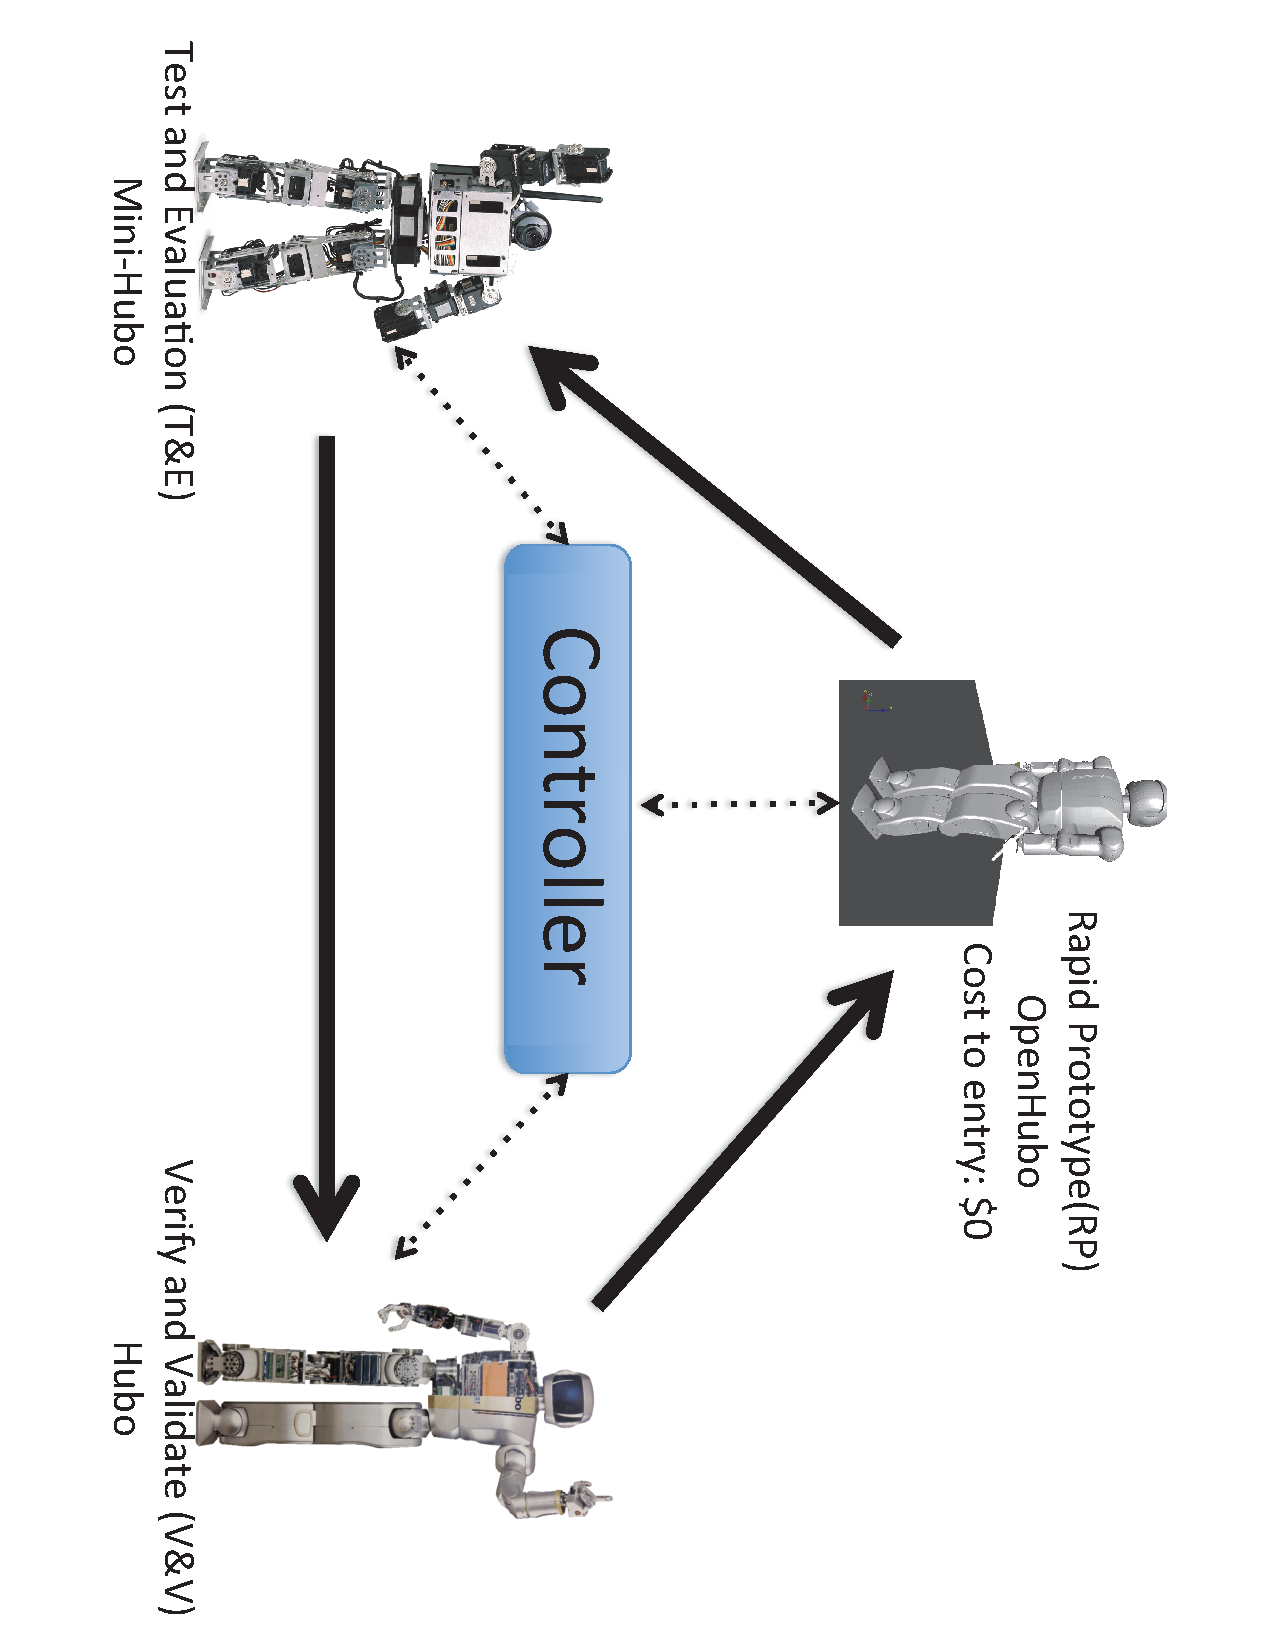
\includegraphics[angle=90, width=0.8\columnwidth]{./pix/threeTier.pdf}
  \caption{Three tier infrastructure. Tier 1: Rapid Prototype (RP) using OpenHubo. Tier 2: Test and Evaluation (T\&E) using Mini-Hubo.  Tier 3: Verify and Validate (V\&V) using Hubo.}
  \label{fig:threeTier}
\end{figure}



